\documentclass[journal]{IEEEtran}
\usepackage{amsmath,amssymb,booktabs,graphicx,microtype,balance}
\usepackage[hidelinks]{hyperref}
\makeatletter
\setlength{\@fptop}{0pt}\setlength{\@fpsep}{6pt}\setlength{\@fpbot}{0pt plus 1fil}
\setlength{\@dblfptop}{0pt}\setlength{\@dblfpsep}{6pt}\setlength{\@dblfpbot}{0pt plus 1fil}
\makeatother
\emergencystretch=2em\sloppy
\title{Coverage-Qualified Evaluation-Contract Auditing for Aerial Vehicle Detection}
\author{Xinling Wen, Jiahao Zhang, Wenqi Liu, Yangxu Ren, and Yu Chen%
\thanks{This work was supported by Henan provincial research, innovation, education-reform, talent, and collaborative-innovation programs (Grant Nos. 241111213000, 26IRTSTHN036, YJS2024JD48, 2025SJGLX086Y, and 254000510003).}%
\thanks{All authors are with the School of Electronics and Information, Zhengzhou University of Aeronautics, Zhengzhou 450046, China. Xinling Wen and Yu Chen are also with the Henan Key Laboratory of General Aviation Technology and the Collaborative Innovation Center of Aeronautics and Astronautics Electronic Information Technology, Henan Province, Zhengzhou 450046, China.}%
\thanks{Corresponding authors: Jiahao Zhang (marchematics@gmail.com) and Yu Chen (chatu@zua.edu.cn).}}
\begin{document}\maketitle
\begin{abstract}
Aerial-detection scores can move because a support rule changes both the target and the treatment of detections near excluded objects. We introduce a coverage-qualified evaluation-contract audit comprising a coverage gate followed by support measurement, an ordered contract path, and common-coverage rank inference. The registered path $A\!\rightarrow\!F\!\rightarrow\!R\!\rightarrow\!S$ changes one evaluator factor at a time and attaches an exact TP/FP/FN ledger to target filtering, removed-object neutralization, and source-ignore handling. At 24 pixels, VisDrone, UAVDT, and AI-TOD retain 73.3\%, 95.1\%, and 9.7\% of valid vehicle boxes. On fixed baseline predictions, their $A\!\rightarrow\!F$ micro-$F_1$ changes are $-.036$, $-.009$, and $-.330$; removed-object neutralization then recovers $.067$, $.004$, and $.080$. AI-TOD covers 66.7\% of images but only 28.2\% of boxes, so its metric replay is explicitly conditional. On 548 common VisDrone images, sequence-paired intervals favor Y11m over ASD for $F_1$ at confidence .25 and for max-$F_1$, but AP50 is unresolved at 24 pixels and favors ASD at normalized .015. The result is a qualified comparison rather than a detector-wide winner claim. An independent AP implementation matches COCOeval at all four checked endpoints.
\end{abstract}
\begin{IEEEkeywords}Aerial detection, annotation support, evaluation contract, coverage qualification, cluster bootstrap.
\end{IEEEkeywords}

\section{Introduction}
A detection score is interpretable only after its evaluation target and matching contract are fixed. This requirement is acute in aerial imagery: a common pixel cutoff can retain almost every vehicle in one source and remove most vehicles in another. Predictions near removed objects may then be counted as false positives or treated as neutral, while source-provided ignore regions add a separate decision. These choices enter the metric before detector outputs are compared.

Cross-dataset bias, heterogeneous label spaces, annotation reliability, and detector error taxonomies are well studied \cite{torralba2011unbiased,zhao2020object,northcutt2021pervasive,bolya2020tide}. Tiny-object procedures can also alter the prediction process itself \cite{akyon2022slicing}. Our question is different: after annotations and prediction caches are fixed, can the evaluator's effect be measured, attributed to explicit contract steps, and separated from sampling uncertainty? Recent GRSL work likewise shows that validation conditions can materially affect remote-sensing conclusions \cite{zhu2025unetmamba,liu2025dem}, but aerial-detection reports rarely connect coverage, support, contract semantics, and rank inference in one record.

Three weaknesses make an unstructured sensitivity sweep hard to defend. First, incomplete prediction coverage can silently change the evaluated population. Second, endpoint ranges do not identify whether movement follows target filtering, the treatment of removed objects, or native ignore regions. Third, a fixed-confidence $F_1$ comparison can confound detector ranking with score calibration, while image-wise resampling can ignore sequence dependence. We address these weaknesses without training another detector.

Our contributions are fourfold. 1) We define a coverage-qualification gate that separates full-dataset annotation support from prediction-covered metric inference. 2) We introduce an ordered evaluation-contract path with an exact count-transition ledger. 3) We replay the same path on VisDrone, UAVDT, and a coverage-conditioned AI-TOD artifact \cite{zhu2018vision,du2018unmanned,xu2022detecting}. 4) We qualify a frozen VisDrone pool with fixed-$F_1$, max-$F_1$, AP50, and sequence-paired cluster intervals. The audit is designed to reveal when a ranking is metric-specific, not to manufacture agreement among metrics.

\section{Coverage-Qualified Contract Audit}
\subsection{Gate 0 and support coordinates}
We use VisDrone2019-DET validation, the UAVDT test split represented in COCO format for a common evaluator, and AI-TOD validation. The available AI-TOD reconstruction includes xView-derived imagery \cite{lam2018xview}. Vehicle mappings are VisDrone \{car, van, truck, bus\}, UAVDT \{car, truck, bus\}, and AI-TOD \{vehicle\}. Raw coverage is established from prediction image names \emph{before} class filtering; a covered image with no retained vehicle prediction is an empty prediction, not a missing observation.

Gate 0 records the annotation denominator, raw coverage, and covered--noncovered differences before any metric is interpreted. Complete artifacts can enter all later layers. An incomplete artifact may enter support diagnosis and a clearly conditioned metric replay, but not a full-benchmark rank claim. We compare AI-TOD coverage groups by boxes per image, support, aspect ratio, and normalized nearest-neighbor spacing; standardized mean differences and Wasserstein distances are released.

Formally, let $\mathcal I_s$ be the registered annotation-image set for source $s$ and $\mathcal P_k$ the image identifiers present in candidate artifact $k$. Its raw coverage is
\begin{equation}
q_{sk}=\frac{|\mathcal I_s\cap\mathcal P_k|}{|\mathcal I_s|}.
\end{equation}
Annotation support is estimated on all of $\mathcal I_s$ and is independent of predictions. A metric endpoint for $k$ is a full-source estimand only when $q_{sk}=1$; otherwise it is written conditionally on $\mathcal J_{sk}=\mathcal I_s\cap\mathcal P_k$. A pairwise rank estimand uses the explicit common set $\mathcal J_{sk\ell}=\mathcal I_s\cap\mathcal P_k\cap\mathcal P_\ell$. This separation prevents a high-coverage artifact from silently redefining the benchmark denominator and prevents unmatched image sets from entering a detector comparison.

For a box $(w,h)$ in image $(W,H)$, absolute and normalized max-side support are
\begin{equation}
s_a=\max(w,h),\qquad s_n=\max\left(\frac{w}{W},\frac{h}{H}\right).
\end{equation}
We register $s_a\in\{16,20,24,28,32,40,48,64\}$ pixels and $s_n\in\{.005,.0075,.010,.015,.020,.030\}$; 24 pixels and .015 are the headline interior values. Under uniform resizing by $\alpha>0$, $s_a'=\alpha s_a$ whereas $s_n'=s_n$. Thus normalized support is resize invariant and absolute support is scale covariant. This property does not imply semantic equivalence across sources; ontology, acquisition geometry, cropping, and density can still differ.

\noindent\textit{Proposition 1 (scale behavior).} Under the uniform transformation $(w,h,W,H)\mapsto(\alpha w,\alpha h,\alpha W,\alpha H)$ with $\alpha>0$, normalized max-side support is invariant and absolute max-side support is covariant. This follows directly because $\max(\alpha w,\alpha h)=\alpha s_a$, whereas both factors of $\alpha$ cancel in $s_n$. The proposition motivates reporting both coordinates; it does not make a shared normalized threshold a claim of semantic equivalence.

\begin{figure*}[!t]
\centering
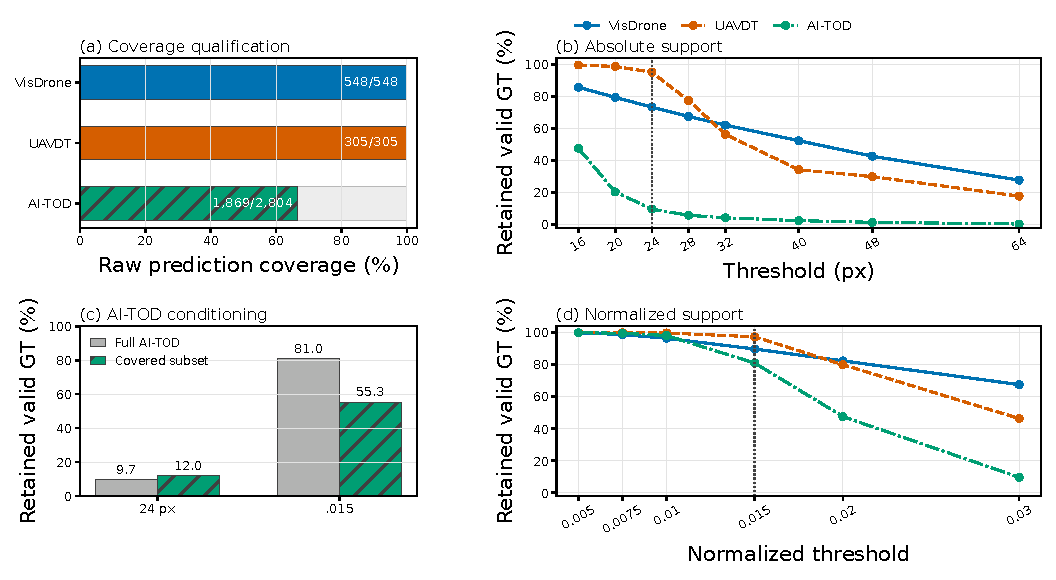
\includegraphics[width=.98\textwidth]{../figures/fig_coverage_qualified_support.pdf}
\caption{Coverage qualification precedes metric interpretation. (a) Raw prediction coverage. (b) Full-source absolute retained-support curves. (c) AI-TOD's covered images contain 28.2\% of its vehicle boxes; its full-source and covered-subset headline support therefore differ. (d) Full-source normalized retained-support curves. Percentages are pooled valid-GT fractions computed before prediction matching.}\label{fig:coverage}
\end{figure*}

\subsection{Ordered contract-path decomposition}
Let $G$ be mapped valid boxes, $G_t\subseteq G$ the boxes retained by support rule $t$, $D_t=G\setminus G_t$ the removed boxes, and $H$ the source-provided ignore regions. We register four contracts as ordered pairs of scored valid and neutral regions:
\begin{align}
\mathcal C_A&=(G,\varnothing), & \mathcal C_F&=(G_t,\varnothing),\nonumber\\
\mathcal C_R&=(G_t,D_t), & \mathcal C_S&=(G_t,D_t\cup H).
\end{align}
$A$ scores all valid boxes with ignore protection off. $F$ filters the target and leaves detections on removed objects eligible as false positives. $R$ keeps the same filtered target but makes removed objects neutral. $S$ then adds source-provided ignores. In every contract, detections are processed by descending score, retained valid GT is matched first, and only an unmatched detection can be neutralized. Ignore overlap follows the COCO crowd denominator, intersection over prediction area, at .5 \cite{lin2014microsoft}.

For metric $m$ at rule $t$, define adjacent path changes
\begin{align}
\delta_{\rm target}&=m_F-m_A, &
\delta_{\rm removed}&=m_R-m_F,\nonumber\\
\delta_{\rm source}&=m_S-m_R.&&
\end{align}
They satisfy the exact path identity
\begin{equation}
m_S-m_A=\delta_{\rm target}+\delta_{\rm removed}+\delta_{\rm source}.
\end{equation}
The associated ledger records the exact $\Delta$TP, $\Delta$FP, and $\Delta$FN at each step. Because $F_1$ is nonlinear, these are path-specific evaluator transitions, not order-free causal effects. The deterministic contract range $C_m(t)=\max_{c\in\{A,F,R,S\}}m_c(t)-\min_c m_c(t)$ remains a compact summary, but it is not a confidence interval.

The path also imposes implementation invariants. Each detection can match at most one scored valid box; scored-valid matching precedes neutralization; and a detection neutralized by $D_t$ or $H$ is neither TP nor FP. For micro-$F_1=2\mathrm{TP}/(2\mathrm{TP}+\mathrm{FP}+\mathrm{FN})$, the ledger is regenerated from image-level integer counts and must close both the count totals and the endpoint identity above. These checks distinguish a semantic contract change from accidental rematching or denominator drift.

\subsection{Metric- and cluster-qualified rank protocol}
The metric layer replays one registered baseline artifact per source at confidence and IoU .25. The rank layer uses five fixed VisDrone configurations with identical 548/548 raw coverage: B-640, B-1280, Y11m, ASD, and Y11n-P2. At terminal contract $S$ and each headline support, we report global micro-$F_1$ at confidence .25, max-$F_1$ over the registered confidence grid $.10$--$.50$, and AP50 with a nontruncating terminal \texttt{maxDets}=2000. AP integrates score ordering and uses IoU .50; max-$F_1$ removes dependence on one confidence operating point while retaining IoU .25.

VisDrone filenames identify 76 sequences. A paired cluster replicate samples 76 sequence identifiers with replacement, includes every image in each sampled sequence, applies identical multiplicities to both configurations, and recomputes pooled TP/FP/FN or pooled-detection AP. We use 10,000 replicates and percentile 95\% intervals. Image-paired results are retained as a supplementary control. Finite-grid boundary cells are exploratory and are not used for confirmatory inference after inspection. Finally, an independent detection-record AP implementation is checked against COCOeval at the two candidates and two headline rules.

The ontology mappings, image denominators, support grid, contract order, headline rules, confidence grid, candidate pool, named top pair, AP cap, sequence definition, bootstrap seed, and replicate count are stored as machine-readable records. Only the two headline supports enter confirmatory pairwise statements. The larger 14-support-by-eight-confidence surface is retained for sensitivity visualization and boundary discovery, not for post-selection pointwise inference.

\section{Results}
\subsection{Coverage and support qualification}
Figure~\ref{fig:coverage} shows full coverage for VisDrone (548/548) and UAVDT (305/305), but 1,869/2,804 images for AI-TOD. At 24 pixels, full-source retained support is 73.3\%, 95.1\%, and 9.7\%; at .015 it is 89.8\%, 97.4\%, and 81.0\%. Normalization narrows the three-source headline spread but does not remove it.

AI-TOD's missingness is support selective. Its covered images are 66.7\% of the validation images but contain 16,900/59,904=28.2\% of vehicle boxes. Covered and noncovered images average 9.0 and 46.0 boxes; their medians are 0 and 21. The covered-subset retained fraction is 12.0\% at 24 pixels and 55.3\% at .015, versus 9.7\% and 81.0\% on the full annotations. AI-TOD therefore passes support diagnosis, but its metric values below describe only the registered covered subset.

The qualification is not triggered by coverage rate alone. Covered versus noncovered images have a boxes-per-image standardized mean difference of $-.673$; at box level, max-side Wasserstein distances are 2.96 pixels and .00370 in normalized units. Consequently, the uncovered part is neither treated as empty prediction nor repaired by weighting. The audit preserves two separate quantities: full-annotation support and covered-subset contract response.

\subsection{Contract-path attribution}
\begin{figure*}[!t]
\centering
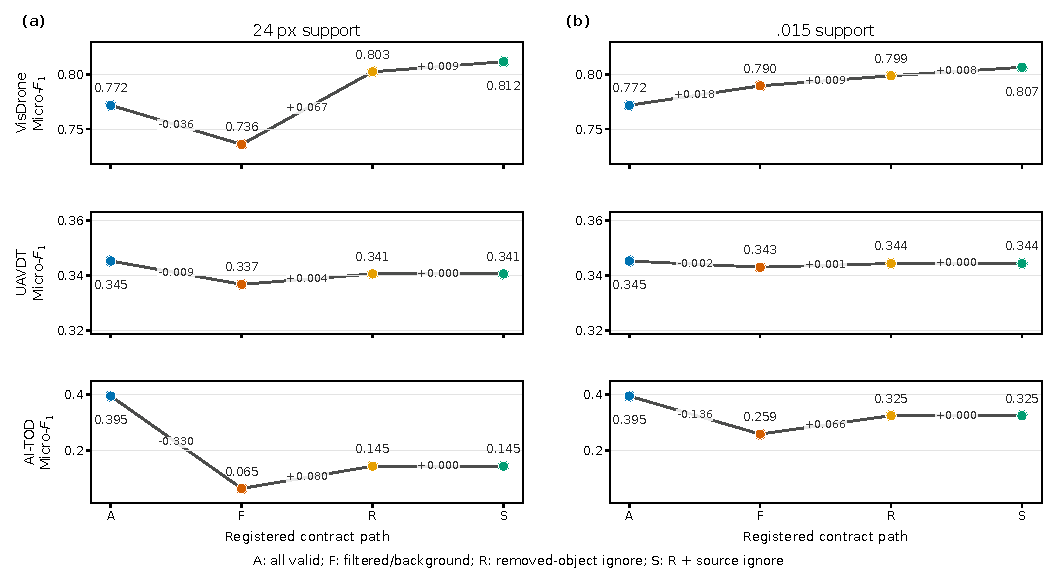
\includegraphics[width=.98\textwidth]{../figures/fig_contract_path_decomposition.pdf}
\caption{Registered $A\!\rightarrow\!F\!\rightarrow\!R\!\rightarrow\!S$ micro-$F_1$ paths for one fixed baseline artifact per source at confidence and IoU .25. (a) Absolute 24-pixel support. (b) Normalized .015 support. Adjacent labels are exact path changes; UAVDT and AI-TOD have no active source-ignore regions, hence $R=S$. AI-TOD values are conditioned on 1,869 covered images.}\label{fig:path}
\end{figure*}

Figure~\ref{fig:path} turns endpoint movement into an evaluator mechanism. At 24 pixels, the VisDrone path is $-.036,+.067,+.009$: filtering initially lowers $F_1$, removed-object neutralization more than recovers that loss, and source ignores add a smaller shift. The count ledger explains the middle step exactly: $F\!\rightarrow\!R$ changes no TP or FN but neutralizes 2,320 false positives. At .015, all three VisDrone steps are positive ($+.018,+.009,+.008$), showing that the sign of target filtering itself depends on the declared support.

UAVDT moves little ($-.009,+.004,0$ at 24 pixels and $-.002,+.001,0$ at .015). AI-TOD behaves differently. Its absolute $A\!\rightarrow\!F$ change is $-.330$, followed by $+.080$ when 30,232 detections near removed objects become neutral; the terminal score remains .145 rather than returning to .395. At .015 the corresponding changes are $-.136$ and $+.066$. Thus the large AI-TOD endpoint range is not solely an artifact of counting detections on removed boxes as background: removed-object handling explains a substantial, separately measured component, while target contraction remains dominant.

Normalized support reduces, but does not eliminate, contract sensitivity in every source. The full four-contract range falls from .076 to .035 for VisDrone, from .0085 to .0023 for UAVDT, and from .330 to .136 for coverage-conditioned AI-TOD. The common direction is consistent with scale invariance, whereas the unequal residual ranges show why normalized support cannot substitute for a source-specific contract audit.

\subsection{Metric- and sequence-qualified ranking}
\begin{figure*}[!t]
\centering
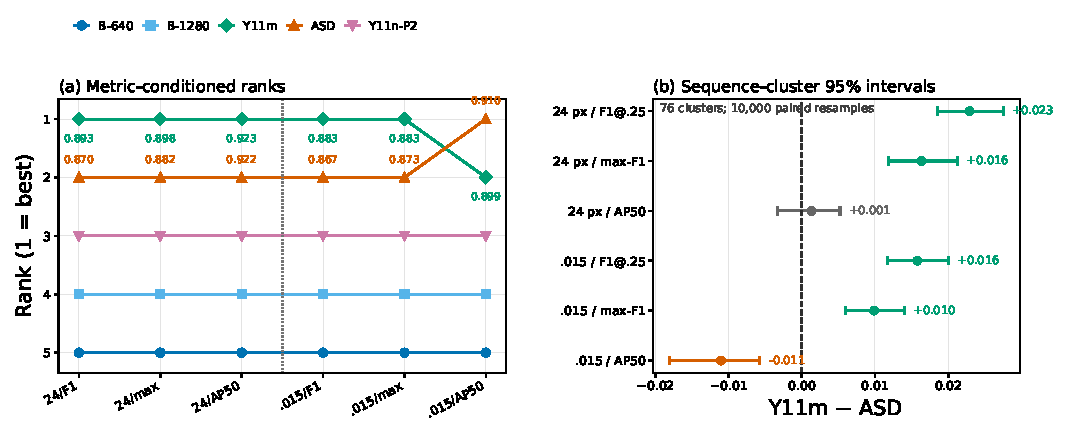
\includegraphics[width=.98\textwidth]{../figures/fig_metric_cluster_qualified_rank.pdf}
\caption{Metric-qualified ranking under terminal contract $S$ on the common 548-image VisDrone set. (a) Ranks and Y11m/ASD point values for fixed-$F_1$, max-$F_1$, and AP50 at both headline supports. (b) Y11m--ASD differences with 95\% intervals from 10,000 paired resamples of 76 filename-derived sequences. Positive values favor Y11m. AP is recomputed from pooled detections in every replicate.}\label{fig:rank}
\end{figure*}

The fixed operating point favors Y11m over ASD at both rules: the absolute difference is .0229 [.0185,.0275], and the normalized difference is .0158 [.0118,.0201]. Reoptimizing each configuration over the registered confidence grid preserves the direction, with max-$F_1$ differences .0163 [.0119,.0213] and .0099 [.0060,.0140]. The operational $F_1$ result is therefore not explained only by the choice of confidence .25.

AP50 prevents a broader winner claim. At 24 pixels, Y11m--ASD is .0013 [$-.0033$,.0052], which is sequence-unresolved. At .015, the difference is $-.0110$ [$-.0181$,$-.0057$], favoring ASD. The stricter localization and score-integrated metric therefore changes the top-pair conclusion even though the lower three ranks remain fixed. This negative result is the purpose of metric qualification: Y11m leads for the registered IoU-.25 $F_1$ objectives, but no detector-wide winner is supported. The custom AP50 values match COCOeval exactly to the reported precision at all four checked endpoints.

\subsection{Evaluator controls}
The registered AP cap is 2,000 detections per image, while the largest observed candidate output is 1,881; headline AP therefore contains no cap-truncated image. This matters because caps of 100 or 300 alter dense aerial-image comparisons even when the winner does not change. For the two candidates and two headline contracts, the independent score-ordered AP calculation and COCOeval agree to machine precision. A separate threshold-first Hungarian replay on the released matching-control subset agrees with greedy matching on the selected winner in all 24 multi-candidate settings; its largest absolute $F_1$ difference is .00546. The matching control validates an aligned component rather than extending the headline rank claim.

Sequence and image resampling also give the same qualitative qualification. The image-paired intervals are [.0186,.0274], [.0122,.0204], and [$-.0035$,.0044] for absolute fixed-$F_1$, max-$F_1$, and AP50, and [.0117,.0199], [.0060,.0136], and [$-.0167$,$-.0078$] for their normalized counterparts. We nevertheless use sequence intervals as the primary record because adjacent VisDrone frames are not exchangeable independent observations.

\balance
\section{Discussion}
The gate, path, ledger, and cluster interval answer different questions. Coverage determines which population is observed. Retained support states which valid target remains. The ordered path attributes deterministic metric movement to one evaluator change at a time. Cross-metric paired intervals then state whether a named configuration comparison is resolved on common sequences. A support shift is not sampling uncertainty, and a resolved $F_1$ margin is not automatically an AP conclusion.

We therefore qualify a rank statement along three independent axes. It is \emph{coverage qualified} only on an explicit common image set, \emph{metric qualified} only for the declared localization and score treatment, and \emph{sampling qualified} only relative to the registered resampling unit. Failure on one axis does not invalidate evidence on the others; it narrows the sentence that can be supported. In this study, Y11m's VisDrone advantage is coverage and sequence qualified for the two IoU-.25 $F_1$ objectives, whereas the AP50 record is unresolved at 24 pixels and reverses at .015. AI-TOD endpoints are contract qualified on covered images but not coverage qualified for the full benchmark.

The path is an audit coordinate system, not a claim that $S$ is universally correct. Applications may choose whether removed valid objects should be background or neutral, but that choice should be explicit and its consequence reported. Likewise, resize invariance makes normalized support comparable under uniform scaling; it does not remove source semantics or acquisition differences. The three-source results empirically demonstrate both points.

The ordered path supplies information that an endpoint band cannot. Comparing $A$ with $S$ alone would merge a target change, a removed-object decision, and native ignore semantics into one number. The intermediate counts show which mechanism dominates and whether a recovery is caused by fewer FN, by neutralized FP, or by both. This attribution is especially important when a support cutoff removes many labeled objects, because a large score response can otherwise be mistaken for model instability or annotation error.

The practical output is a compact audit record rather than a preferred universal threshold. It contains the annotation denominator and prediction coverage; retained support in absolute and normalized coordinates; contract endpoints and integer count transitions; the exact common set and metric definition used for each comparison; and paired uncertainty at the source's dependence unit. These fields make two studies comparable even when they choose different valid application contracts. They also expose when an apparent robustness claim comes from a saturated detection cap, an incomplete prediction cache, a fixed confidence calibration, or image-wise resampling of correlated frames.

The evidence remains artifact scoped. AI-TOD has no full-benchmark metric or rank inference; VisDrone conclusions concern five frozen configurations; sequence clusters are derived from filenames; and no transition estimates annotation-error rates or causal detector effects. Full threshold records, the 18-row count ledger, coverage diagnostics, image-paired intervals, matching and cap checks, and replay instructions appear in the supplementary material and released repository: \url{https://github.com/Marchematics/aerial-evaluation-audit}.

\section{Conclusion}
Coverage-qualified contract auditing converts a support-rule sensitivity check into a reproducible evaluation method. It identifies the observed population, measures support, decomposes target and ignore semantics with exact count transitions, and qualifies common-coverage ranks across metrics and sequence dependence. The resulting record explains large score movement without overstating a detector winner.

\bibliographystyle{IEEEtran}\bibliography{references}
\end{document}
